\documentclass[11pt]{article}
\usepackage{amsmath,amssymb,booktabs,graphicx}
\usepackage[margin=1in]{geometry}
\begin{document}
\section*{LS-RBF Parameter-Mesh Jacobian Diagnostics}
This note documents the Jacobian checks added to the LS primary-mode selection stage for the RBF manifold pipeline.
\subsection*{0. Command used}
\begin{verbatim}
python3 stage7a_prepare_rbf_dataset_ls.py --n-primary 3 --basis-dir stage_2_pod_rve --train-dir stage_1_training_set_fom --out-dir stage_7_ann_data_ls --mesh-name rve_geometry --plot-max-samples 110000 --jacobian-mesh-type delaunay --jacobian-mesh-max-points 6000 --jacobian-mesh-seed 42
\end{verbatim}
\subsection*{1. Deformation-factor matrix}
We define a diagonal deformation-factor (scaling) matrix to normalize the parameter domain before meshing:
\begin{equation}
\boldsymbol{\xi} = \mathbf{D}_{\mu}(\boldsymbol{\mu}-\boldsymbol{\mu}_c),\qquad \mathbf{D}_{\mu} = \mathrm{diag}\!\left(\frac{2}{\Delta \mu_1},\frac{2}{\Delta \mu_2},\frac{2}{\Delta \mu_3}\right).
\end{equation}
This reduces anisotropy in the parameter cloud and improves numerical robustness of the mesh and local Jacobians.
\subsection*{2. Parameter mesh and map Jacobians}
A 3D Delaunay tetrahedralization is built in the normalized parameter space. For each tetrahedron $e$, using four corresponding actual states in $(\mu,q_m)$, we compute a local affine map $q_m\approx \mathbf{A}_e\mu+\mathbf{b}_e$.
\begin{equation}
\mathbf{A}_e = \mathbf{Q}_e\mathbf{M}_e^{-1},\qquad \mathbf{M}_e=[\mu_a-\mu_0\ \mu_b-\mu_0\ \mu_c-\mu_0],\quad \mathbf{Q}_e=[q_a-q_0\ q_b-q_0\ q_c-q_0].
\end{equation}
We monitor: (i) $\det(\mathbf{M}_e)$ for parameter-mesh degeneracy, and (ii) $\det(\mathbf{A}_e)=\det(\partial q_m/\partial\mu)$ for local folding.
\subsection*{3. Physical deformation Jacobian}
For each applied Green-Lagrange strain sample, we compute $F=\sqrt{2E+I}$ and monitor $\det(F)$ to check local admissibility of the macro deformation.
\subsection*{4. Run summary}
\begin{center}
\begin{tabular}{ll}
\toprule
Quantity & Value \\
\midrule
$N_\text{mesh nodes}$ & 5940 \\
$N_\text{cells}$ & 39086 \\
mesh type & delaunay \\
mesh cell type & tet \\
negative $\det(J_\mu)$ count & 0 \\
negative $\det(\partial q^{LS}/\partial\mu)$ count & 564 \\
$\min |\det(J_\mu)|$ & 1.001803e-20 \\
$\min\det(\partial q^{LS}/\partial\mu)$ & -3.019476e+08 \\
$\min\det(F)$ & 7.937254e-01 \\
$\max\det(F)$ & 5.000000e+00 \\
\bottomrule
\end{tabular}
\end{center}
\subsection*{5. Deformation-factor matrix used}
\begin{equation}
\mathbf{D}_{\mu}=\mathrm{diag}\left(9.523810e-01,9.523810e-01,1.000000e+01\right)\end{equation}
\begin{align}
\mu_c &= \left(9.500000e-01,9.500000e-01,0.000000e+00\right),\\
\Delta\mu &= \left(2.100000e+00,2.100000e+00,2.000000e-01\right).
\end{align}
\subsection*{6. Figures}
\begin{figure}[h!]
\centering
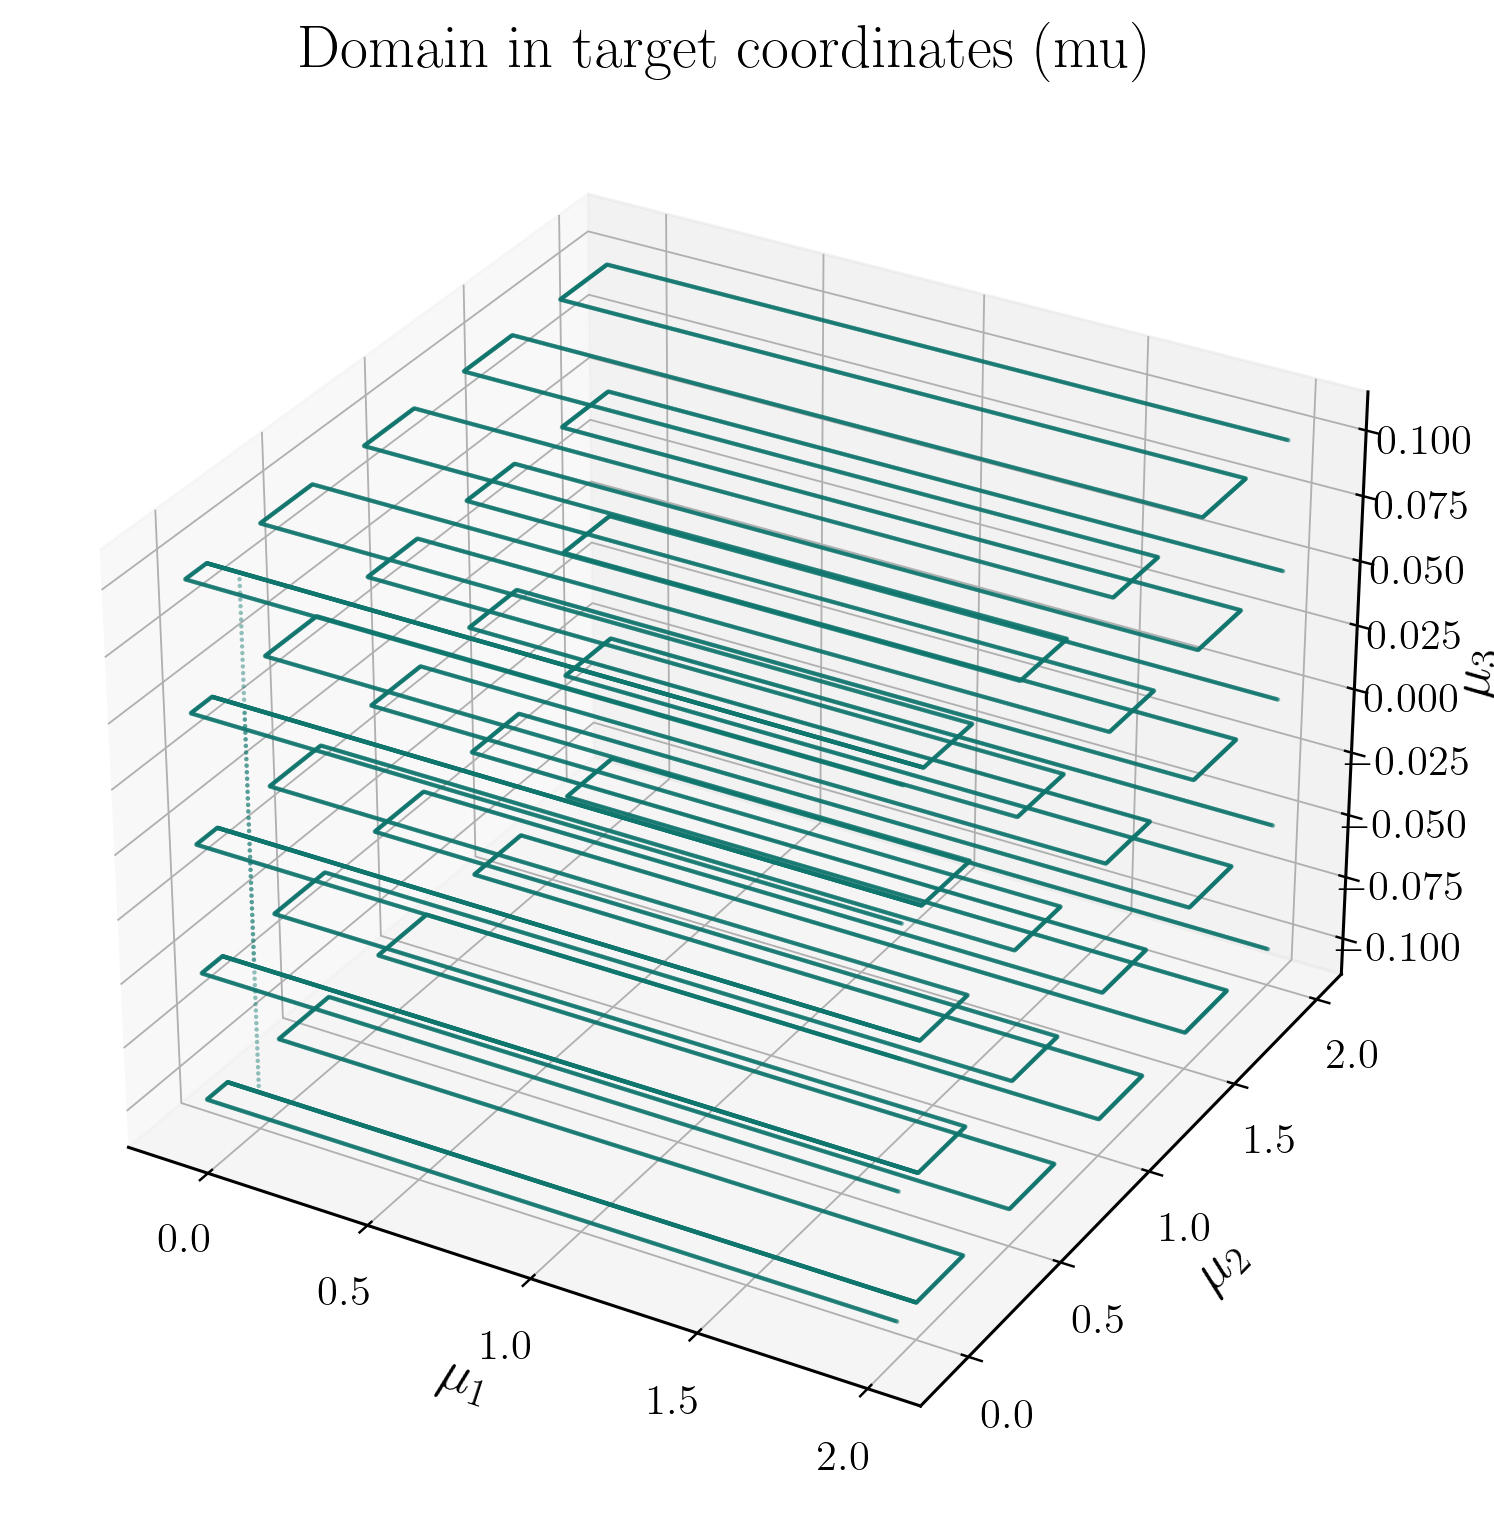
\includegraphics[width=0.48\textwidth]{domain_mu_targets_3d.png}
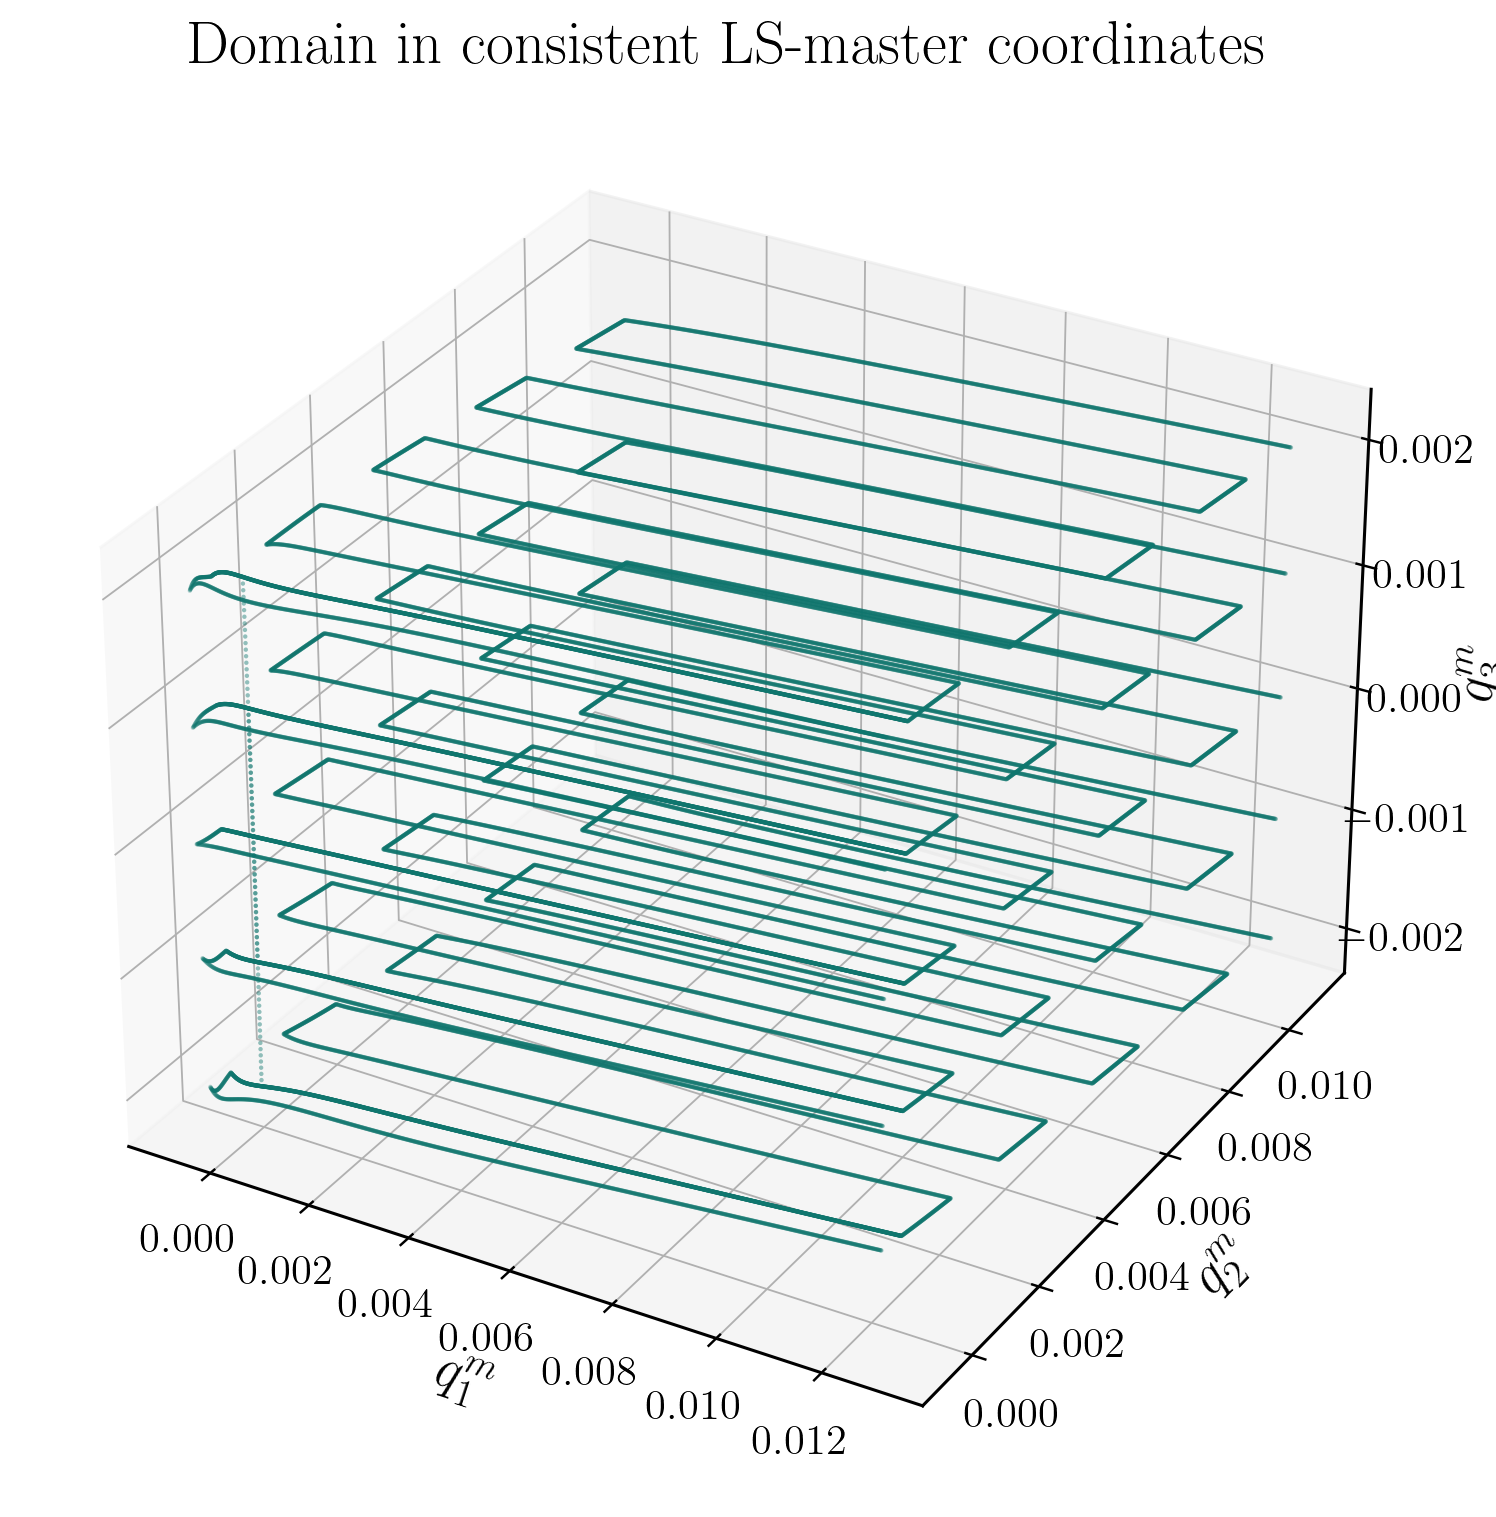
\includegraphics[width=0.48\textwidth]{domain_qm_first3_3d.png}
\caption{Point clouds in physical parameter space and consistent LS-master space.}
\end{figure}
\begin{figure}[h!]
\centering
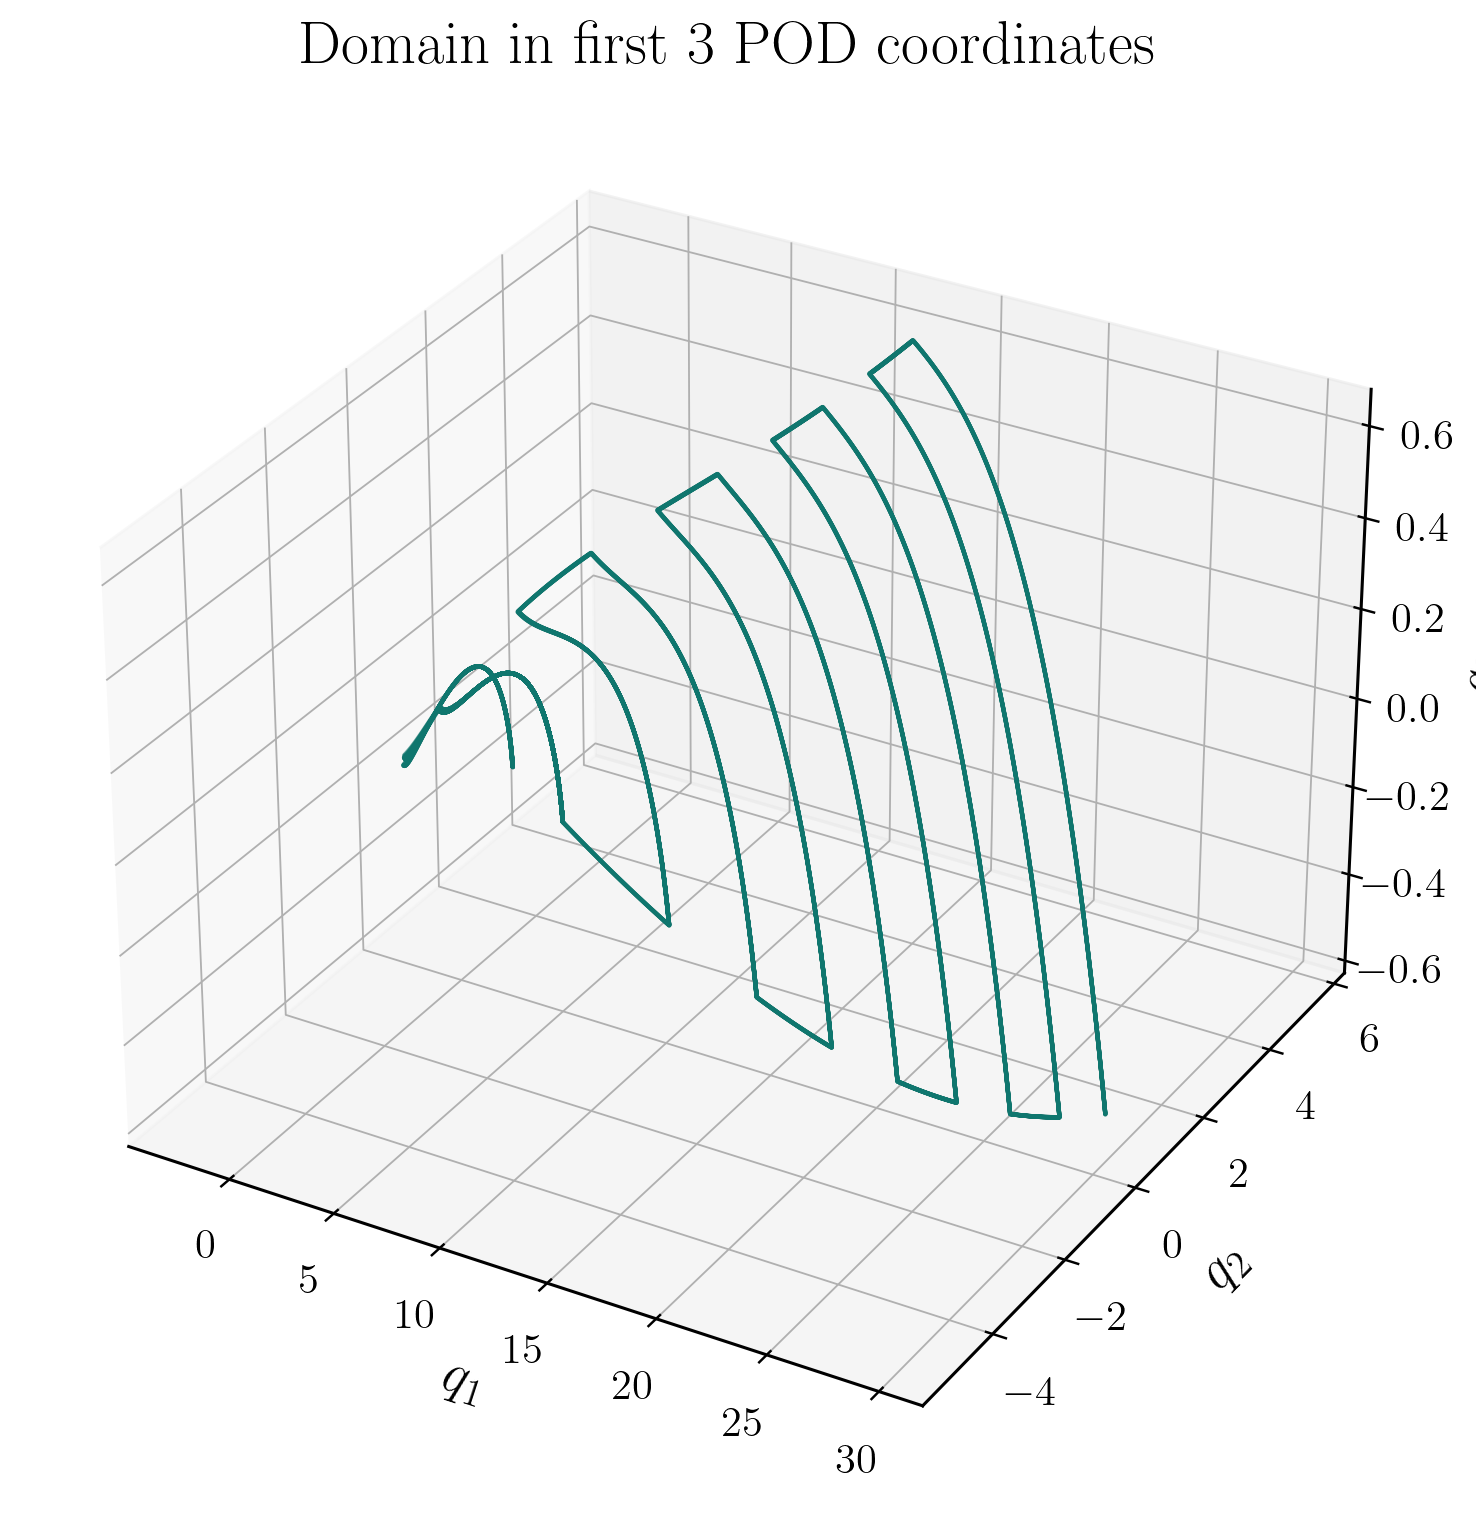
\includegraphics[width=0.48\textwidth]{domain_qpod_first3_3d.png}
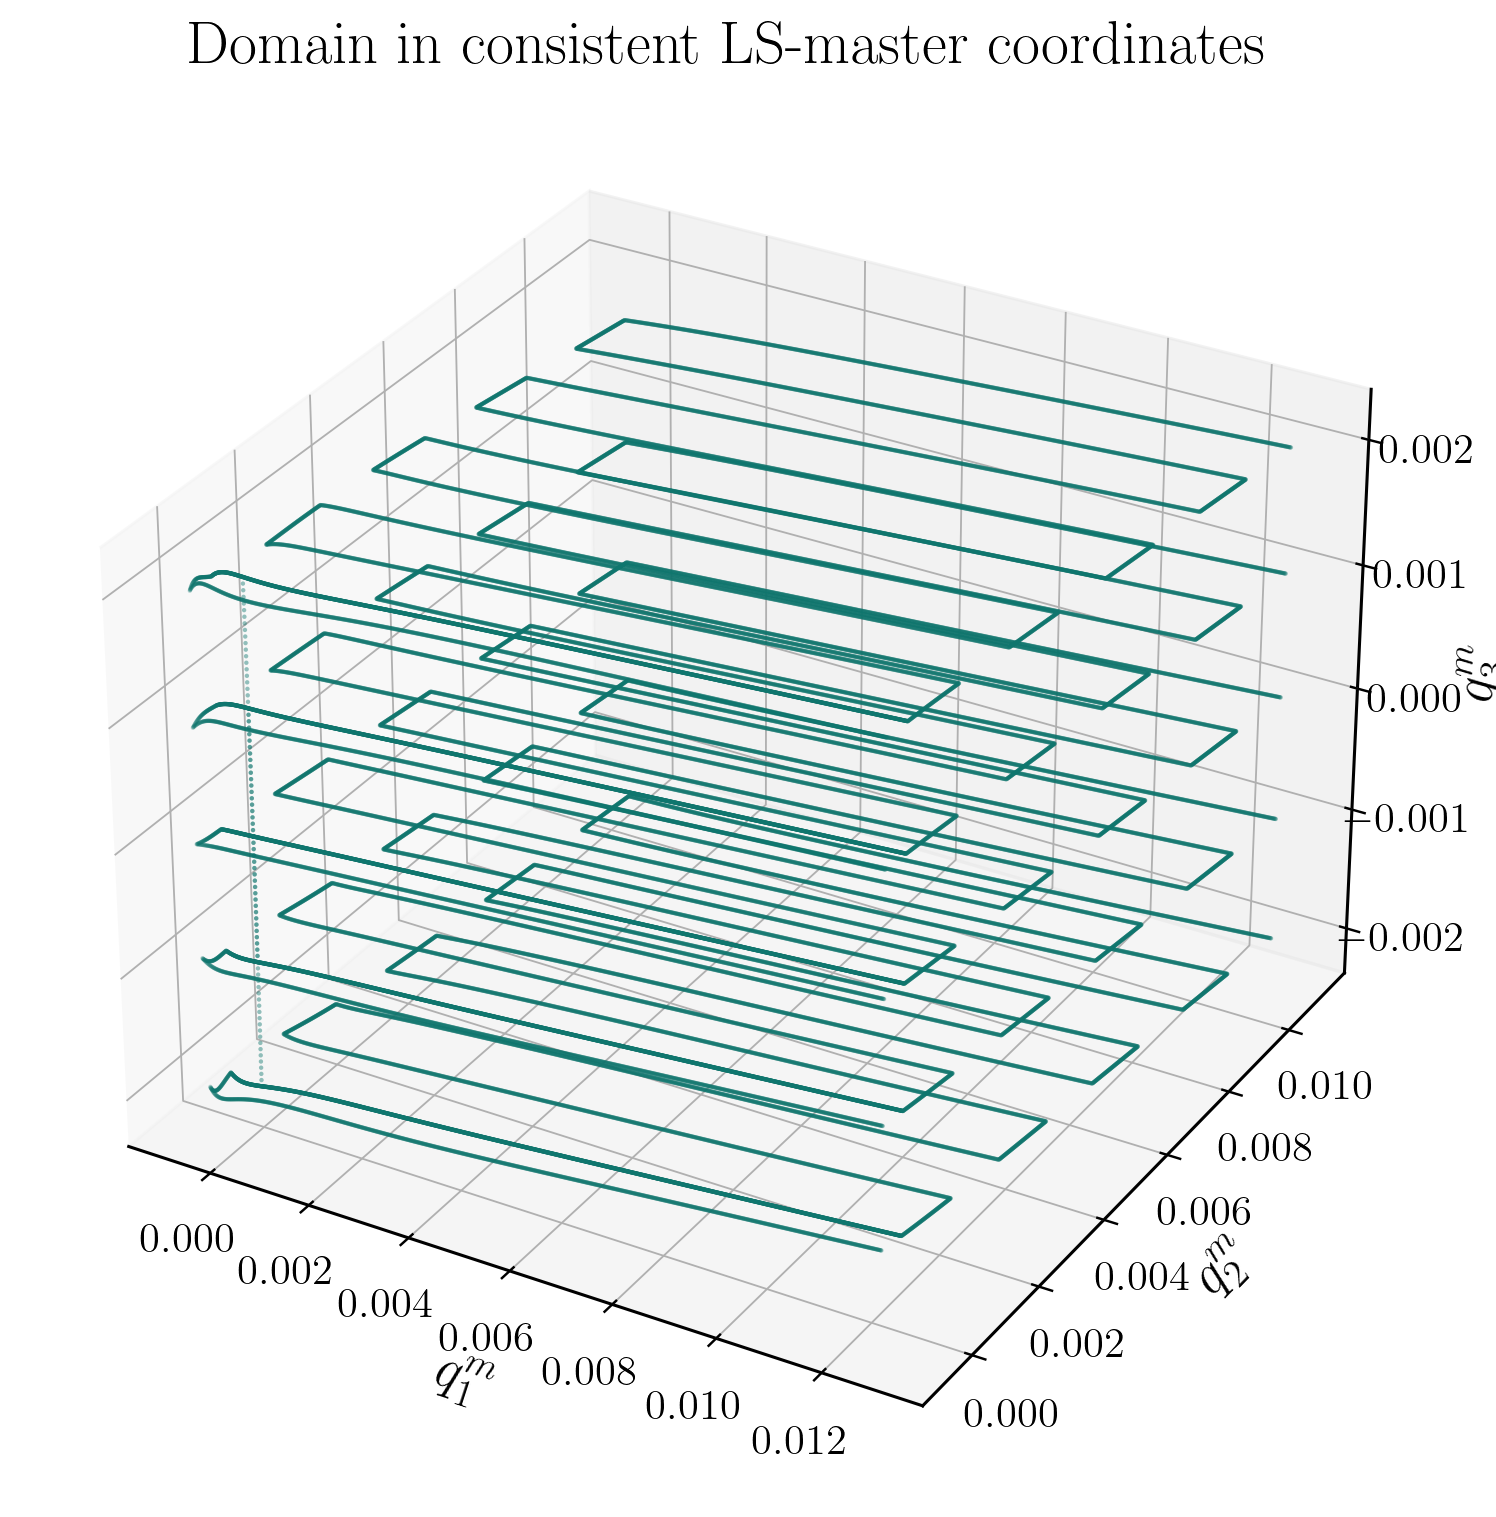
\includegraphics[width=0.48\textwidth]{domain_qm_first3_3d.png}
\caption{Point clouds in POD-first-3 and consistent LS-master coordinates.}
\end{figure}
\begin{figure}[h!]
\centering
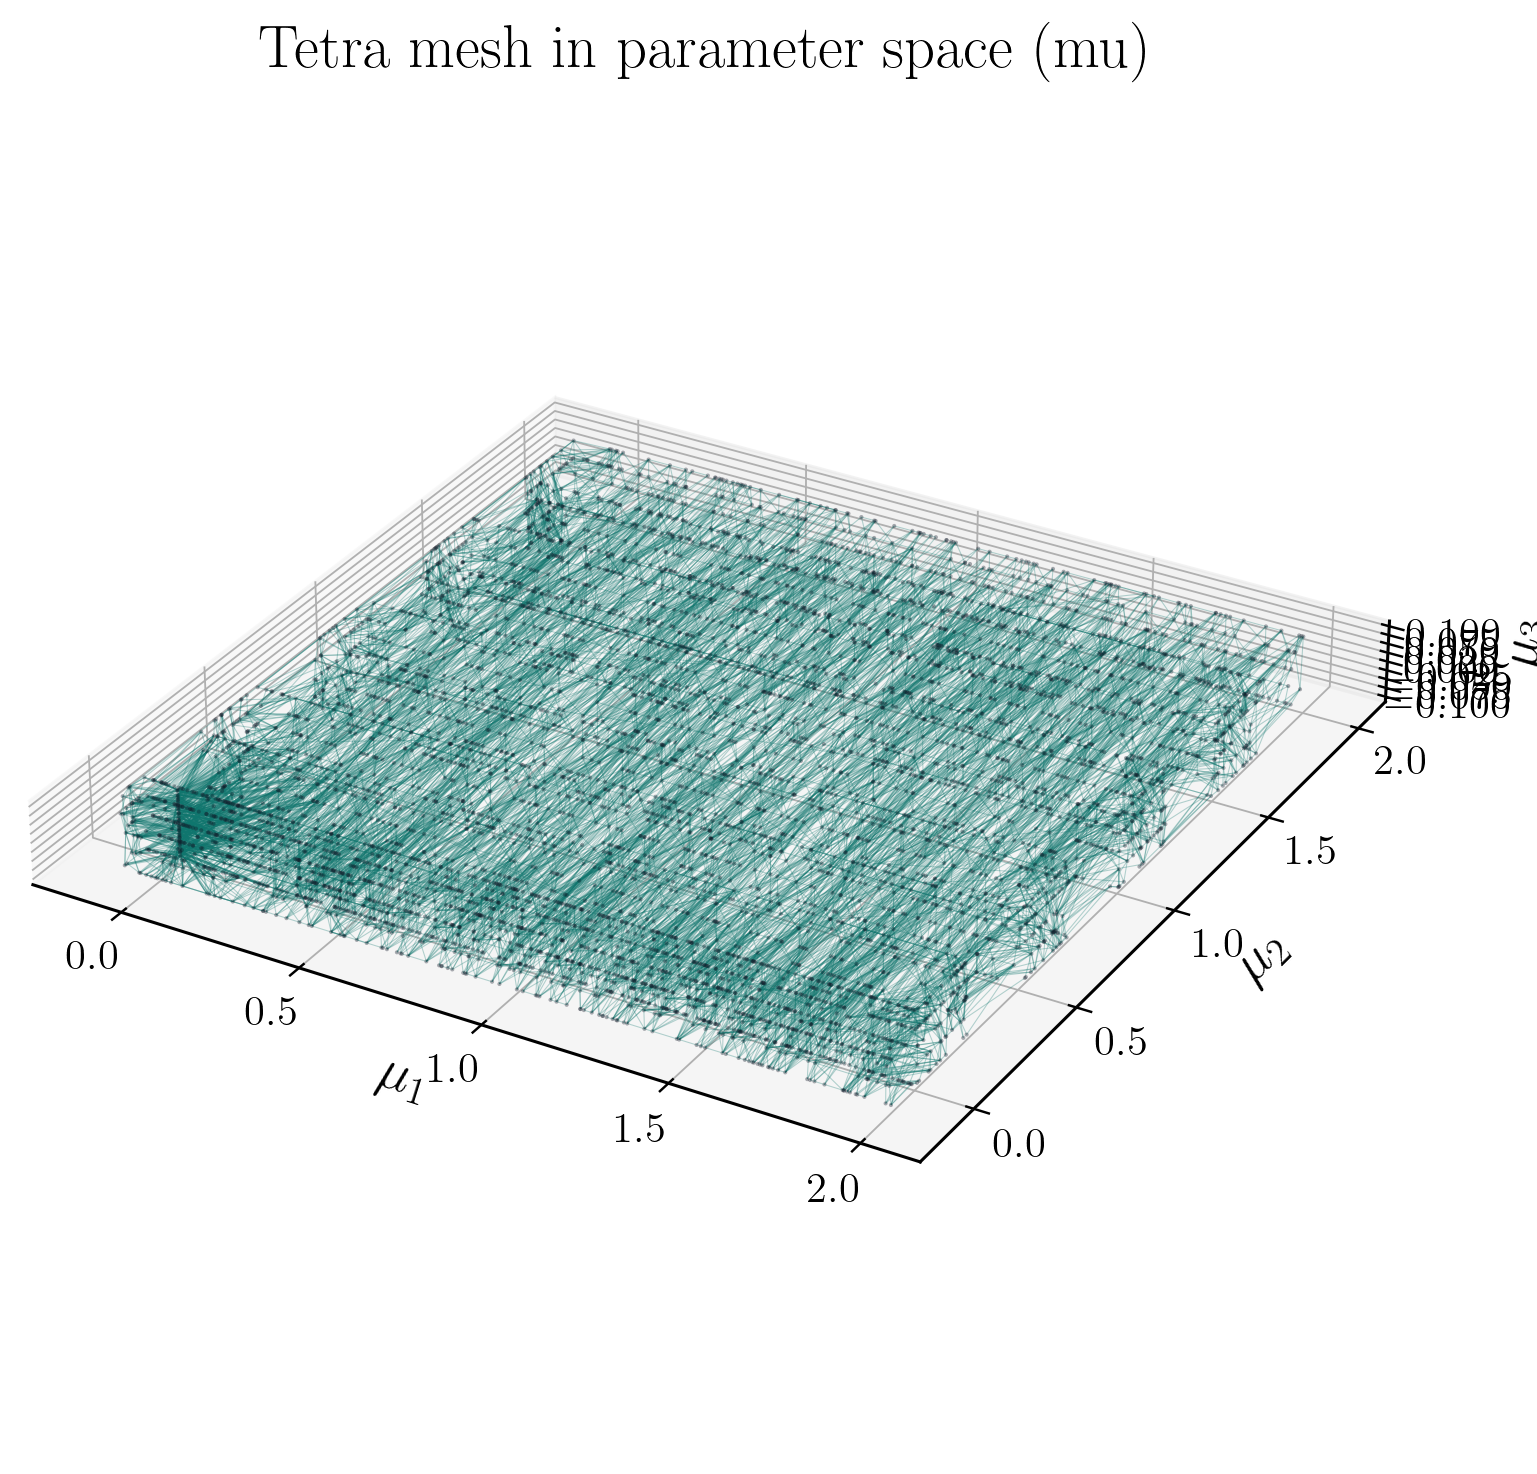
\includegraphics[width=0.48\textwidth]{parameter_mesh_mu_edges_3d.png}
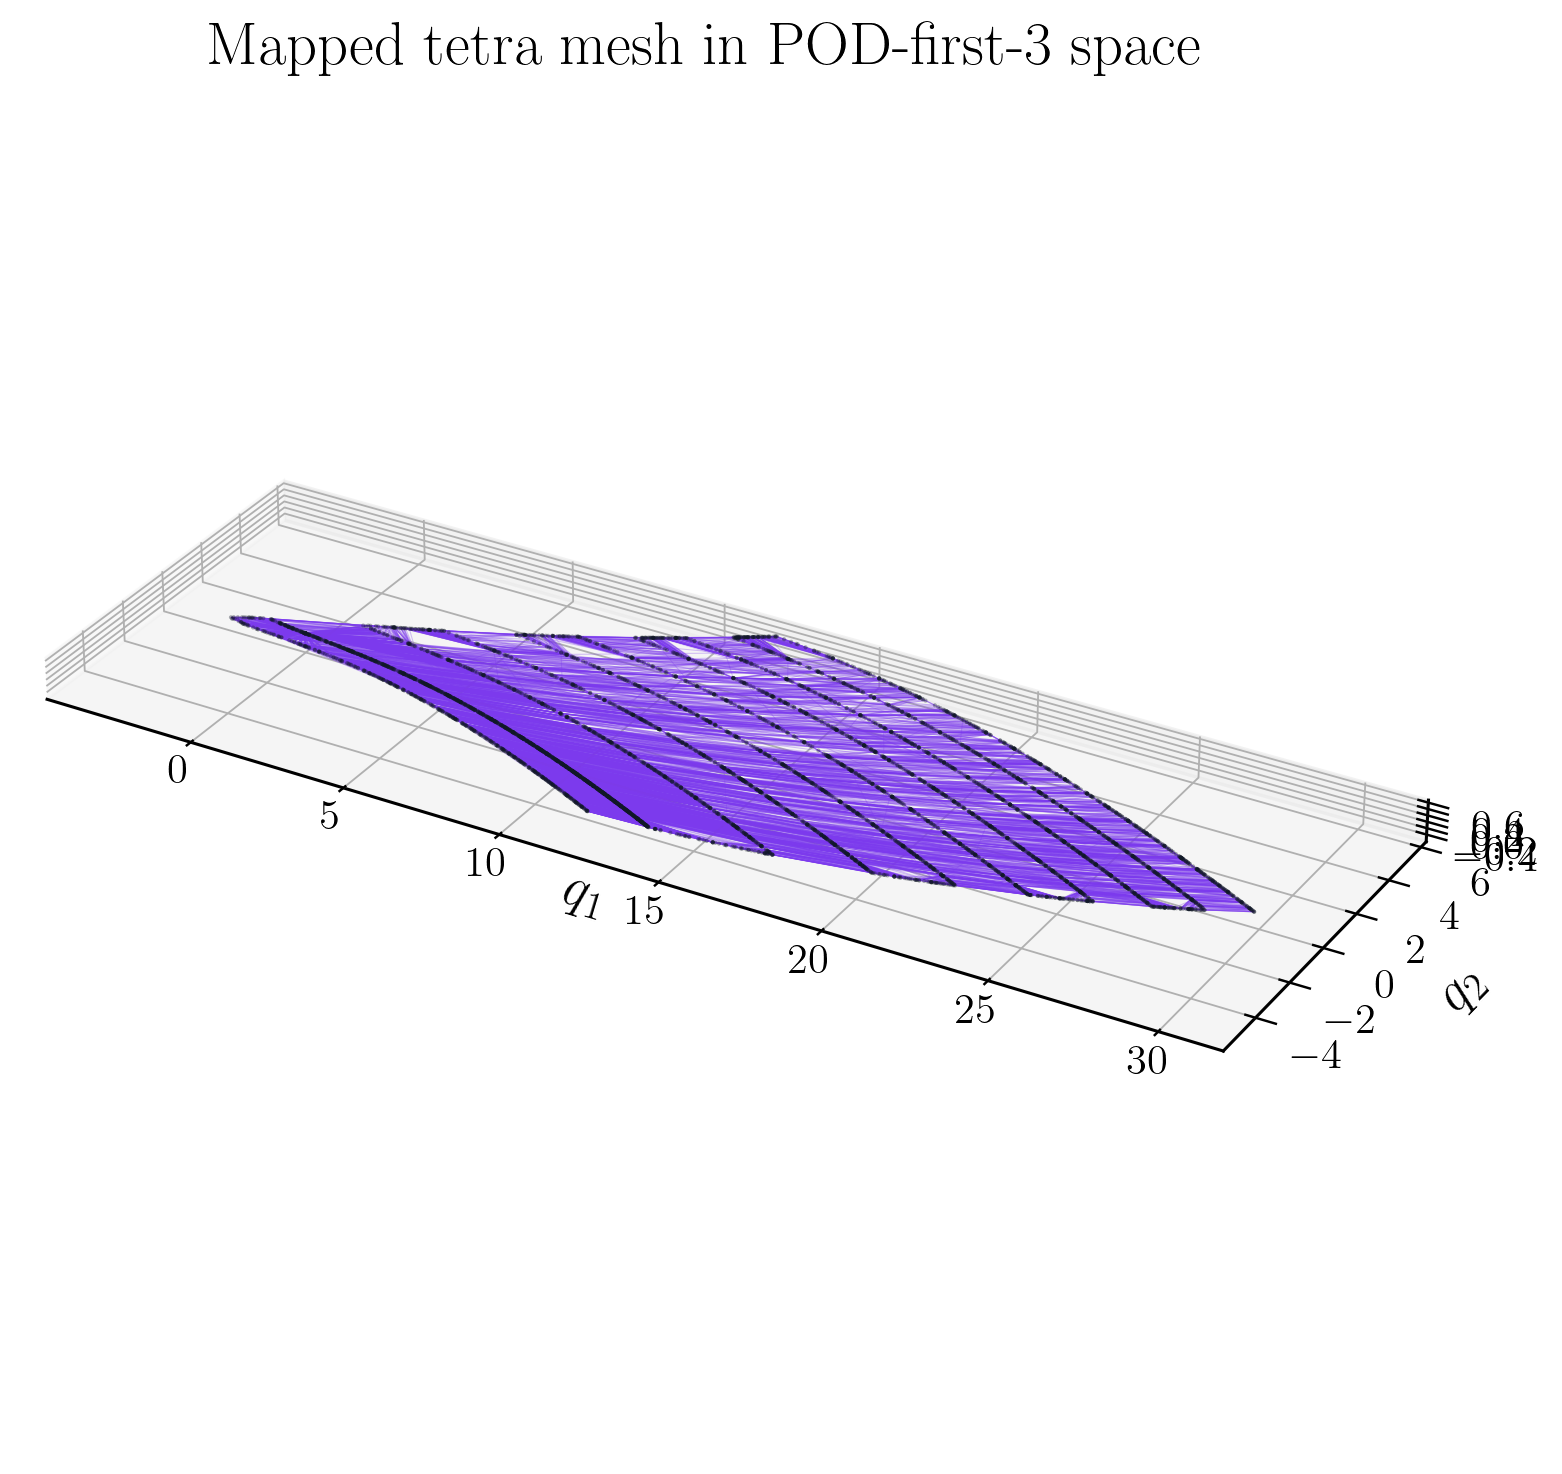
\includegraphics[width=0.48\textwidth]{parameter_mesh_q_pod_edges_3d.png}
\caption{Parameter-mesh edges and mapped POD-first-3 mesh edges.}
\end{figure}
\begin{figure}[h!]
\centering
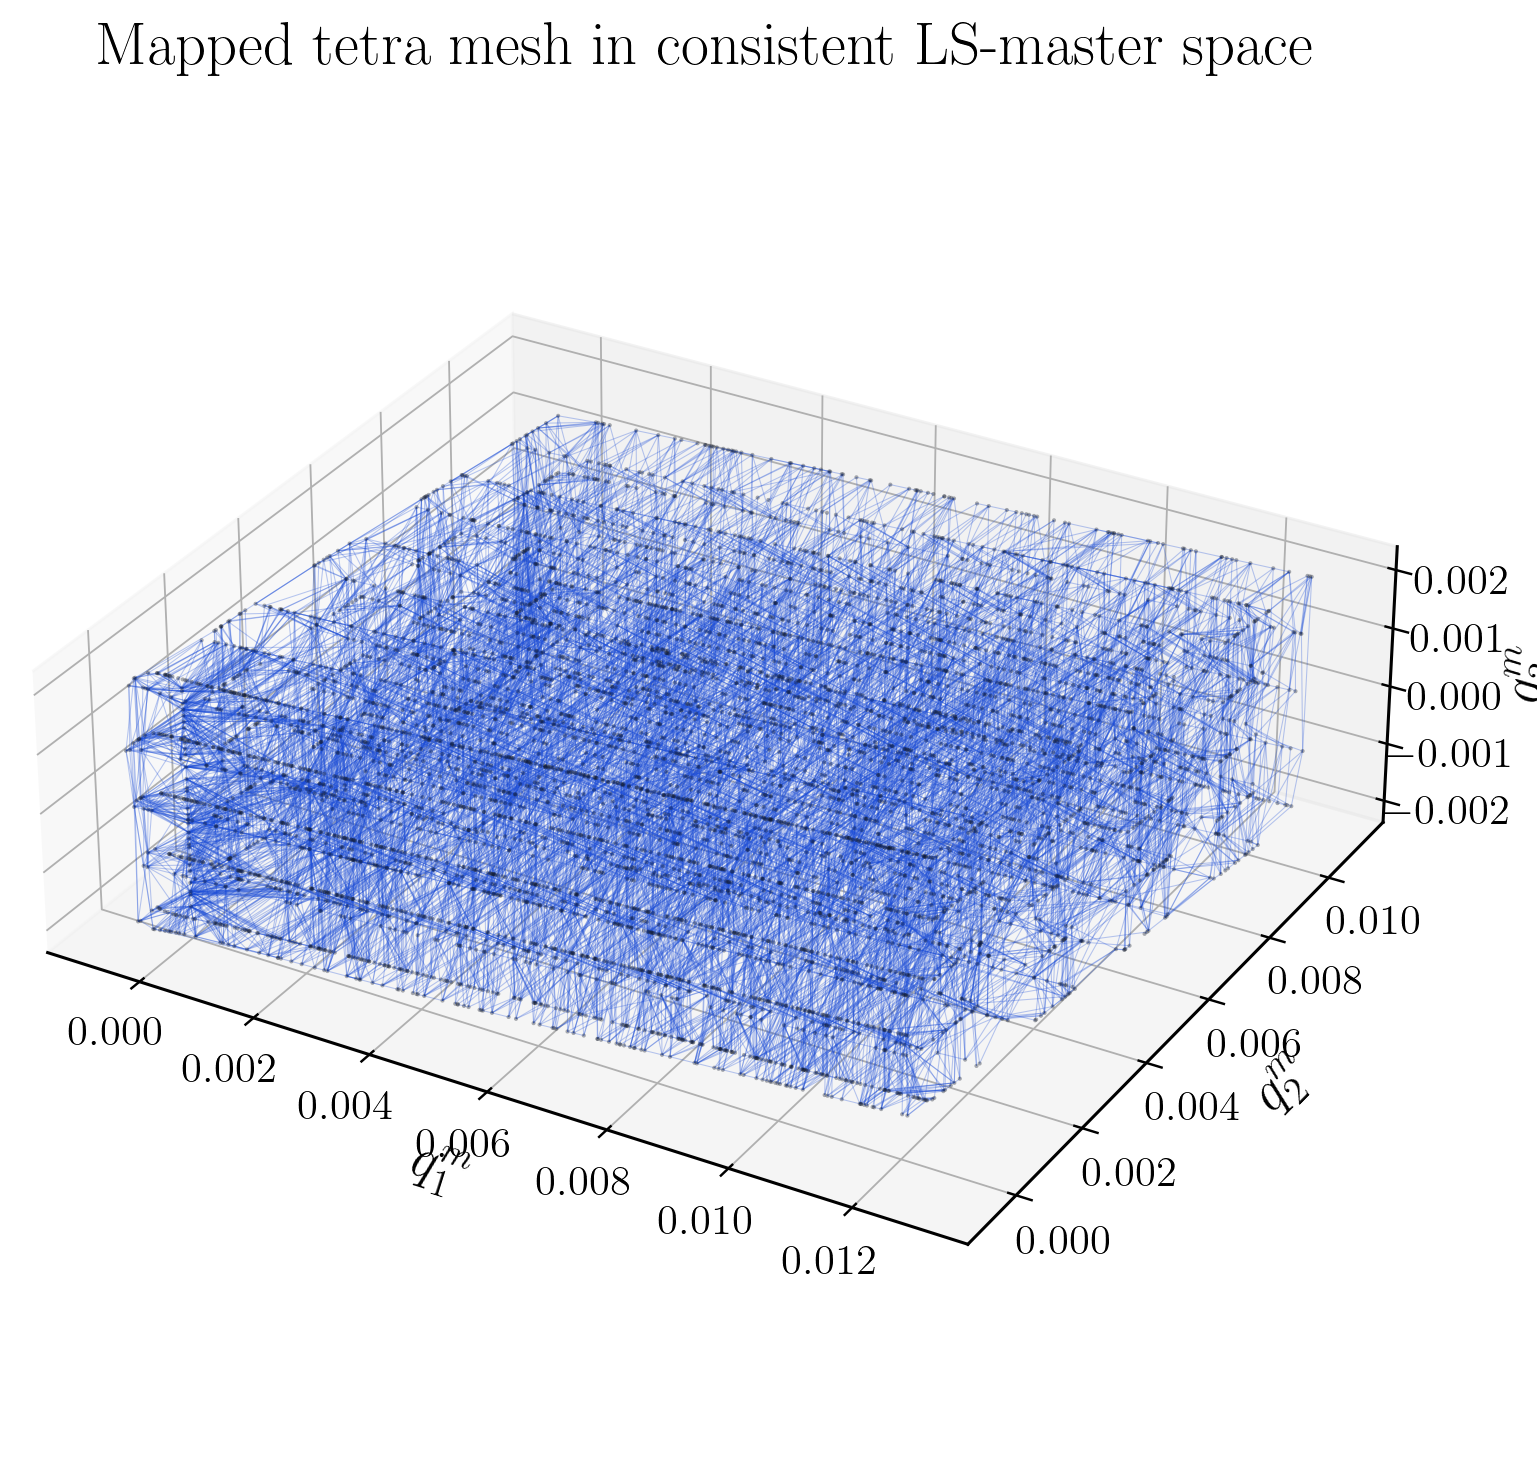
\includegraphics[width=0.48\textwidth]{parameter_mesh_q_m_edges_3d.png}
\caption{Delaunay parameter-mesh edges mapped to consistent LS-master space.}
\end{figure}
\begin{figure}[h!]
\centering
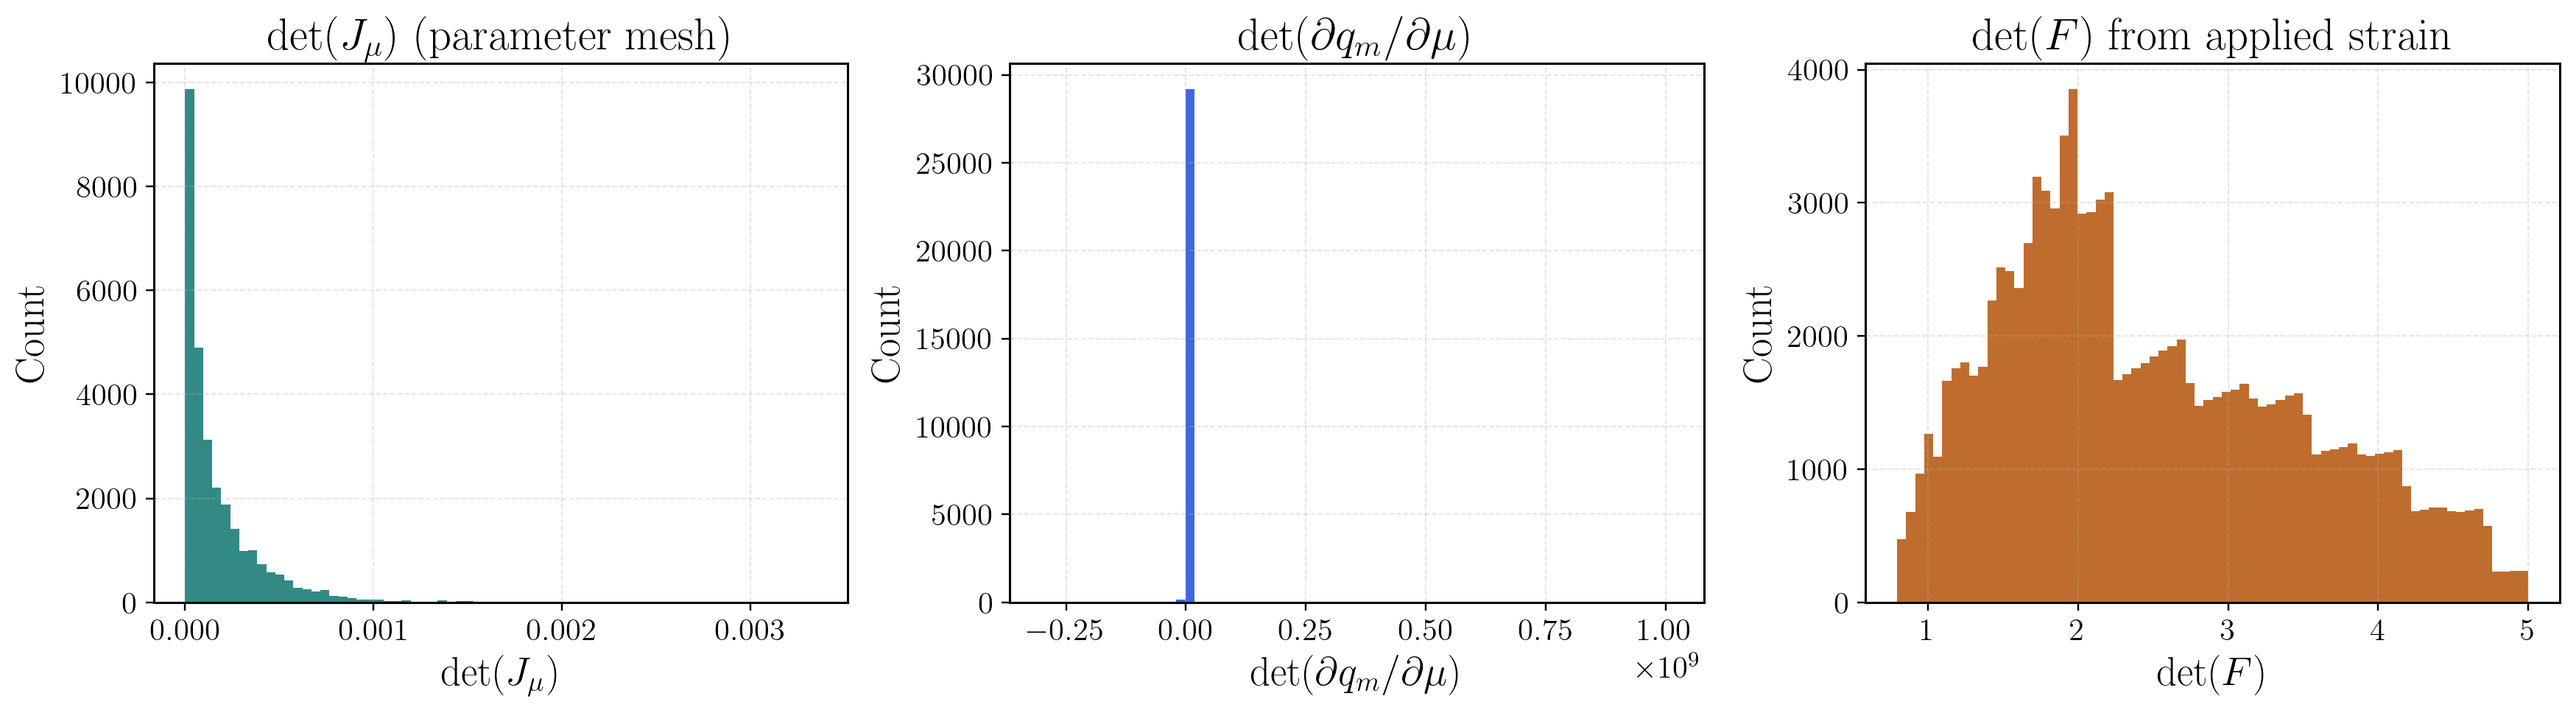
\includegraphics[width=0.70\textwidth]{jacobian_histograms_ls_rbf.png}
\caption{Histograms of parameter-cell, mapping, and physical Jacobians.}
\end{figure}
\end{document}
